\documentclass[letterpaper,11pt]{article}
\usepackage[margin=1in]{geometry}
\usepackage{courier}
\usepackage{graphicx}
\graphicspath{ {./images/} }

\begin{document}
\title{
	\Huge{Problem Set 4}\\
	\Large{MIT 6.0002}\\
	\large{Introduction to Computational Thinking and Data Science\\
	as Taught in Fall 2016}
}
\author{
	John L. Jones IV
}
\maketitle
\pagebreak
\section*{Trends of Simulation A and Simulation B}
\begin{enumerate}
	\item What happens to the total population before introducing the antibiotic?
		\\ Without an antibiotic the bacteria will reproduce until the maximum population is reached. See Figure 1. 
	\item What happens to the resistant bacteria population before introducing the antibiotic?
		\\ The resistant bacteria population will grow, but also compete with the non-resistant bacteria. See Figure 2. 
	\item What happens to the total population after introducing the antibiotic?
		\\ The total population will rapidly decrease after the antibiotic is introduced. See Figure 2 and 3.
	\item What happens to the resistant bacteria population after introducing the antibiotic?
		\\ It may actaully see a small increase in population size, see Figure 2.
		Or, all bacteria may no longer be fit to survice, see Figure 3.
\end{enumerate}

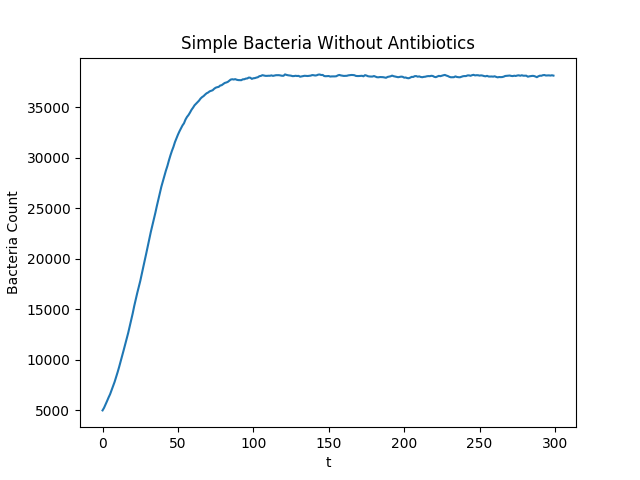
\includegraphics{Figure_1}
\center{Figure 1. Simple Simulation Without an Antibiotic.}

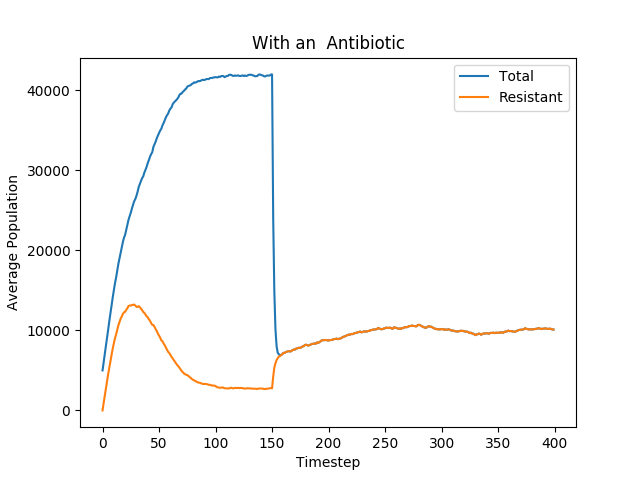
\includegraphics{Figure_2}
\center{Figure 2. Simulation 'A' With Antibiotic.}

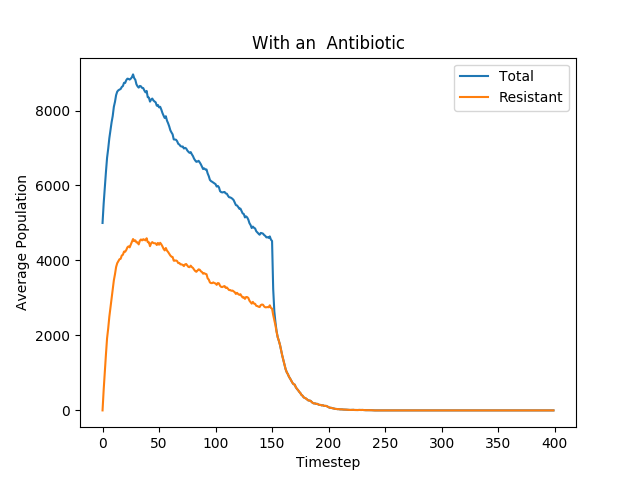
\includegraphics{Figure_3}
\center{Figure 3. Simulation 'B' With Antibiotic.}

\end{document}
